\begin{frame}
\frametitle{Additional simulation and analysis}       
\begin{textblock*}{12.5cm}(0.1cm,2.2cm) % {block width} (coords)
	\begin{figure}[ht!] % replace 't' with 'b' to force it to 
		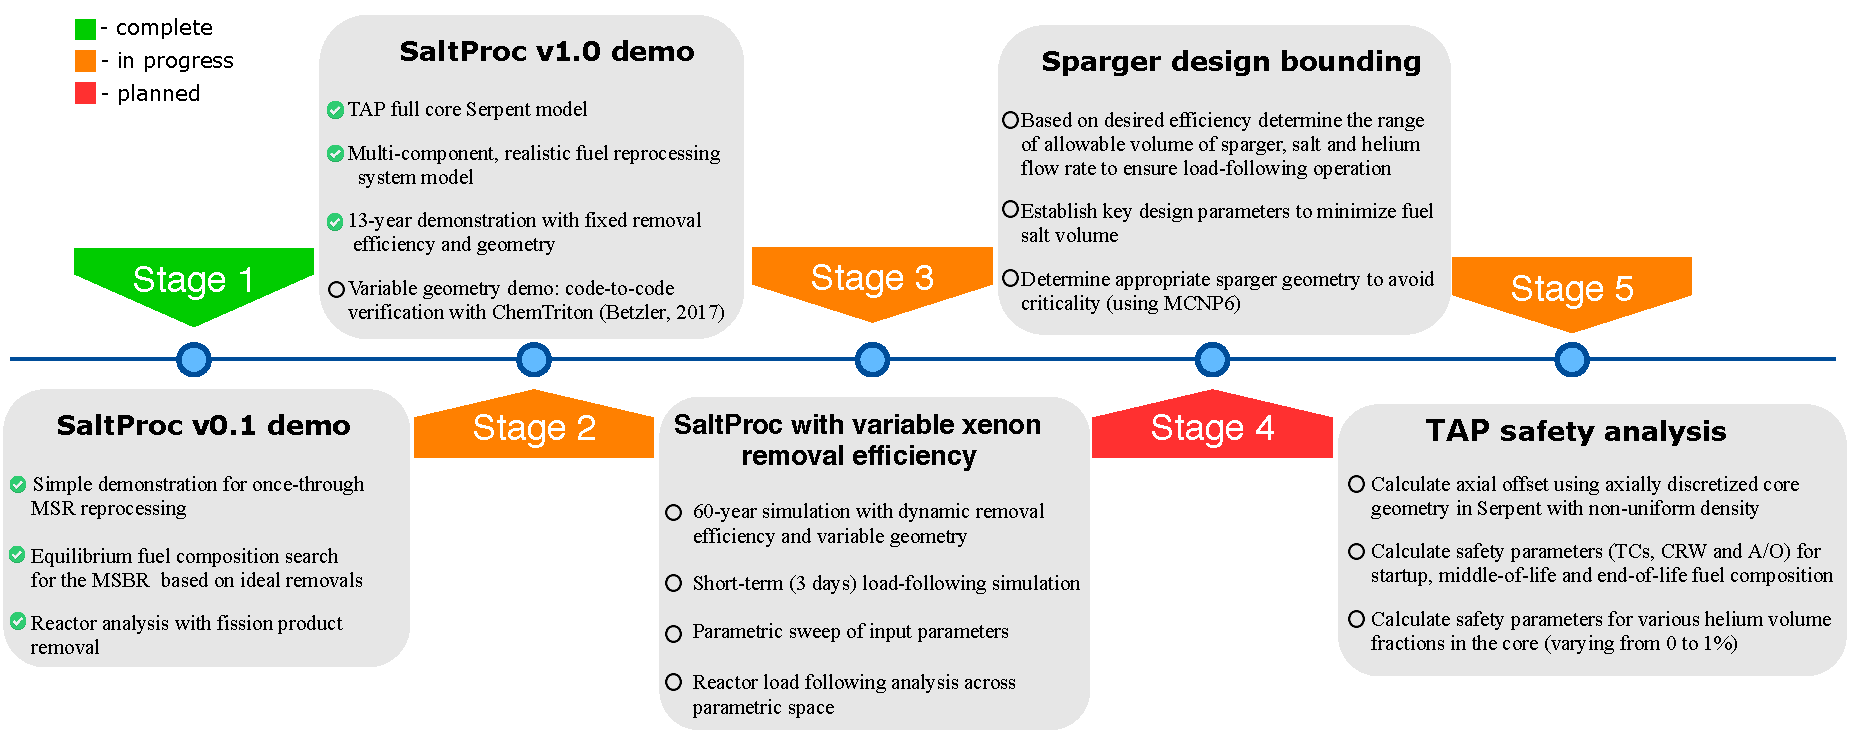
\includegraphics[width=\textwidth]{./images/progress_chart.pdf} 
	\end{figure}
\end{textblock*}
\end{frame}


\begin{frame}
\frametitle{SaltProc demonstration for realistic on-line reprocessing system}
	\begin{block}{Finishing Stage 2}
		\begin{enumerate}
			\item Implement variable core geometry capability in SaltProc
			\item Demonstrate a key feature of
the \gls{TAP} reactor - 
			adjusting the moderator rod configuration - which is necessary to 
			maintain
the reactor criticality during the 60-years lifetime.
			\item Perform life-time long depletion simulation using SaltProc 
			and compare obtained results with Betzler \emph{et al.} 
			\cite{betzler_assessment_2017}
		\end{enumerate}
	\end{block}
	
	\begin{block}{Stage 3}
		\begin{enumerate}
			\item Incorporate extraction efficiencies as a function of many 
			physical system design
parameters (e.g., void fraction in the 
			salt, helium bubble size)
			\item Perform life-time long depletion simulation with dynamic 
			removal efficiency
			\item Perform short-term (3 day) depletion in load-folowing regime
		\end{enumerate}
	\end{block}
\end{frame}
